\documentclass[a4paper,12pt]{book}
\usepackage[utf8]{inputenc}
\usepackage{amsmath,amssymb,latexsym}
\usepackage{graphicx,subfigure}
\usepackage{tcolorbox}
\usepackage{wrapfig}
\usepackage{rotating}
\usepackage[margin=2.5cm]{geometry}
\newtheorem{Equation}{\indent Equation}[section]
\textwidth=6in
\renewcommand{\baselinestretch}{1.5}


\begin{document}
\pagenumbering{gobble}

\begin{sidewaysfigure}
%\begin{figure}[h!]
  \begin{center}
    \subfigure{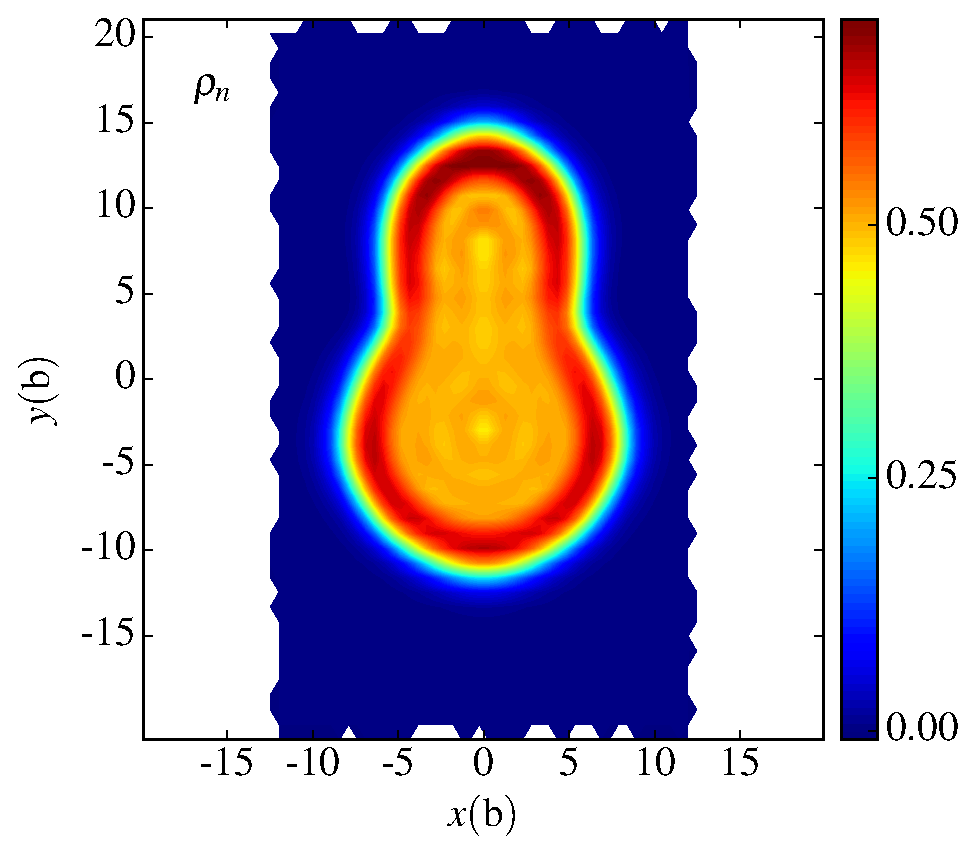
\includegraphics[width=0.3\linewidth]{294Og-140024n-locali.eps}}\label{fig:294Og-140024n-locali}
    \subfigure{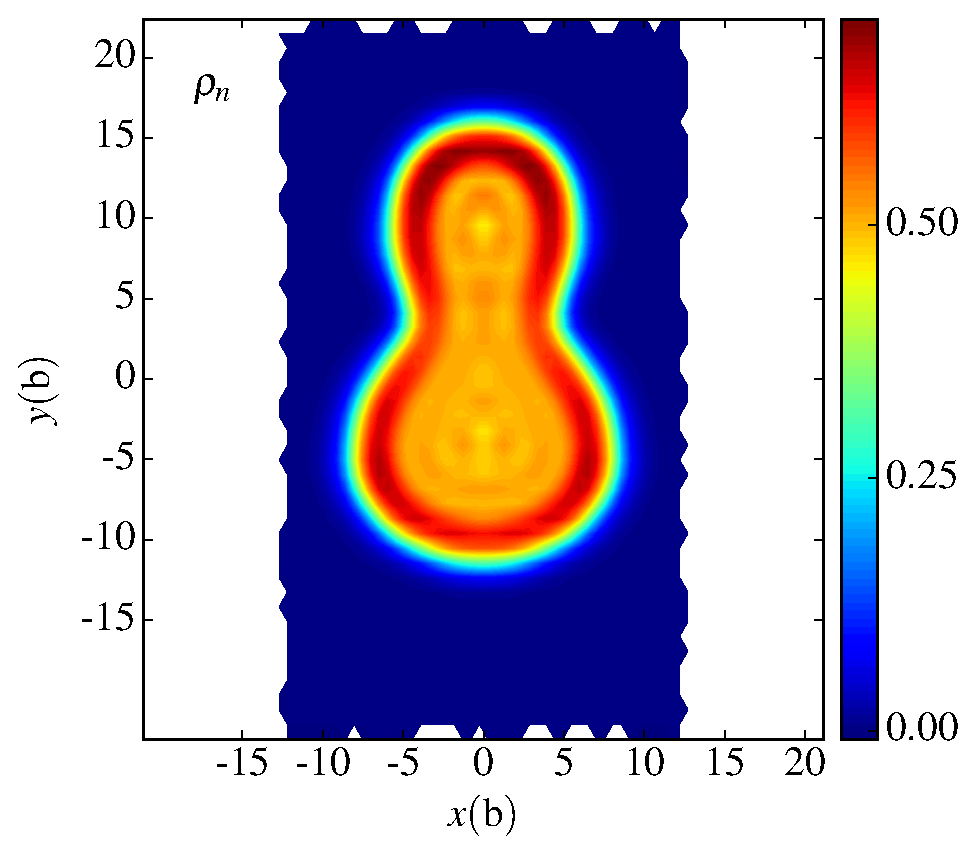
\includegraphics[width=0.3\linewidth]{294Og-200044n-locali.eps}}\label{fig:294Og-200044n-locali}
    \subfigure{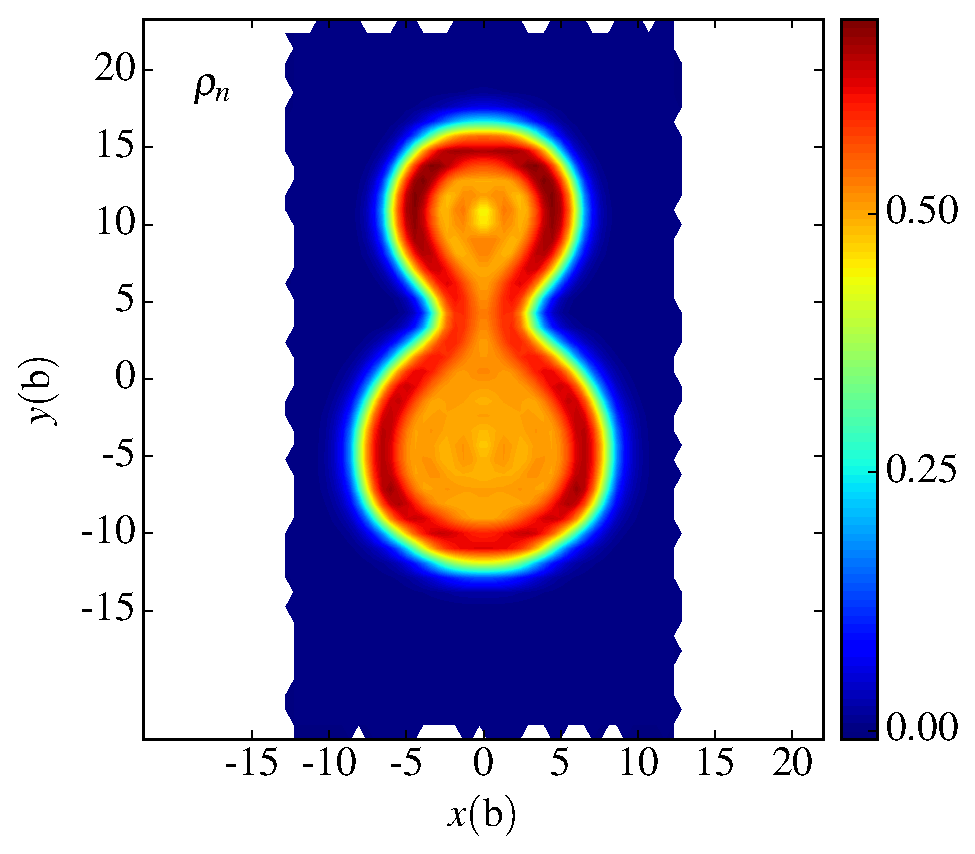
\includegraphics[width=0.3\linewidth]{294Og-264060n-locali.eps}}\label{fig:294Og-264060n-locali}
    \subfigure[$Q_{20}=140 b, Q_{30}=24 b^{\frac{3}{2}}$ (just beyond the outer turning point)]{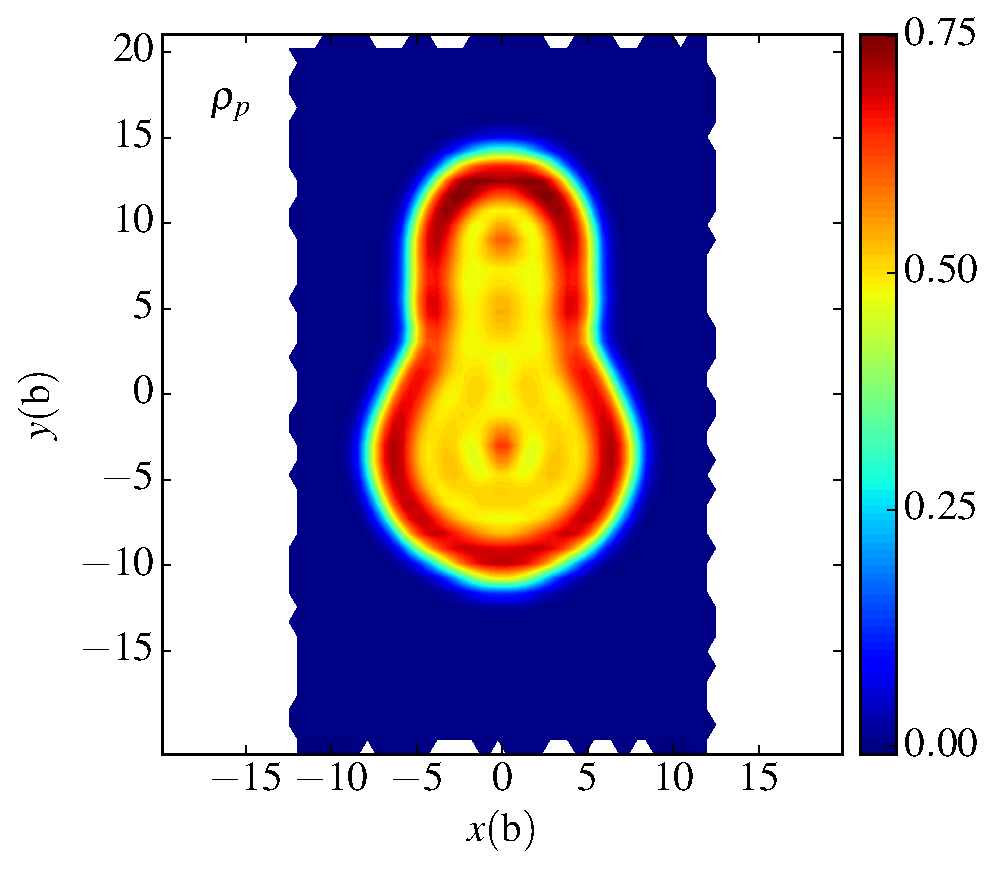
\includegraphics[width=0.3\linewidth]{294Og-140024p-locali.eps}}\label{fig:294Og-140024p-locali}
    \subfigure[$Q_{20}=200 b, Q_{30}=44 b^{\frac{3}{2}}$]{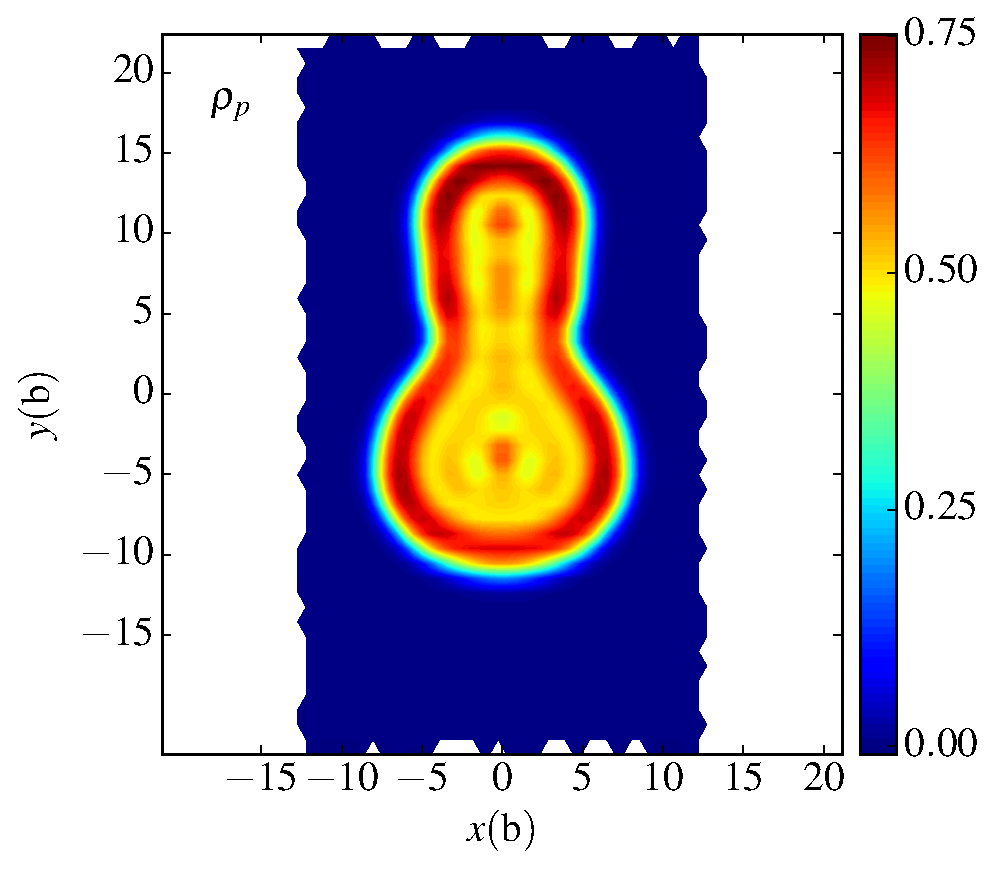
\includegraphics[width=0.3\linewidth]{294Og-200044p-locali.eps}}\label{fig:294Og-200044p-locali}
    \subfigure[$Q_{20}=264 b, Q_{30}=60 b^{\frac{3}{2}}$ (just before scission)]{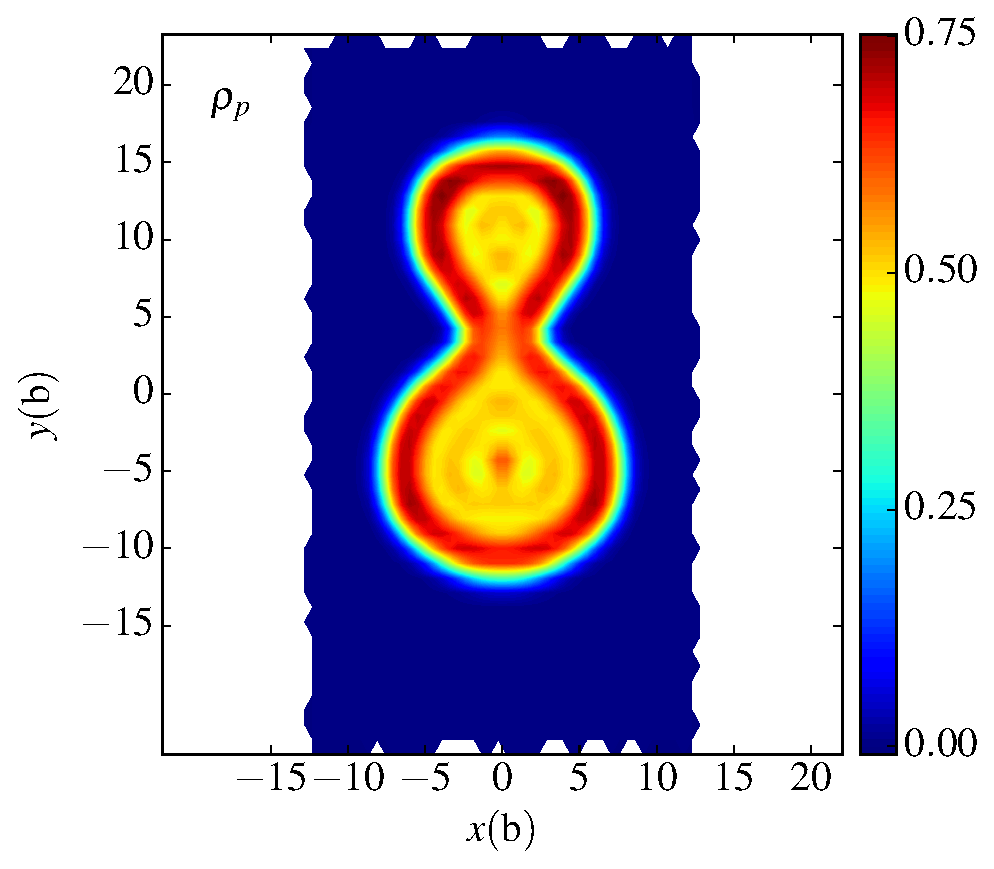
\includegraphics[width=0.3\linewidth]{294Og-264060p-locali.eps}}\label{fig:294Og-264060p-locali}  \end{center}
  \caption{\textbf{Top}: Neutron spatial localization for $^{294}$Og. Shells are already starting to develop as early as just beyond the scission point. \textbf{Bottom}: Proton spatial localization for $^{294}$Og. Note that the lead proton shell starts to develop early, but the krypton proton shell doesn't develop until much later}
%\end{figure}
\end{sidewaysfigure}

\end{document}